\chapter{Timing Analysis and Anomalies}

\section{Evolution of TA-definitions}

A timing anomaly (TA) is a situation where a local favorable condition leads to a globally worse state (for example, a cache hit leading to slowdown of the program).  The notion of timing anomalies dates back to 1999 when they were first introduced by Lundqvist and Stenstr\"om \cite{lundqvist_timing_1999} in context of timing analysis. Basically, TA is a feature of an architecture which makes it hard to analyze timing behavior properly. Such anomalies may have a tremendous impact on execution time which is not captured by the WET analysis. Especially dangerous is so-called domino effect, also discovered by Lundqvist and Stenstr\"om. It leads to an unbounded slowdown effect of the TA.

Despite the fact that timing anomalies have been known for a long time, the exact TA definition is a subject to debates. Since 1999 several attempts were made to formalize the notion of TA, some of them being more focused on the exact microarchitecture (like \cite{gruin_minotaur_2023}) and some being more abstract and general (like \cite{binder_definitions_2022}, \cite{hahn_design_2020}). In this section we are giving an overview of existing definitions comparing their strengths and weaknesses.

\subsection{Step Heights}

Gebhard \cite{gebhard_timing_2012} gives a timing-anomaly definition based on local execution time of instructions in comparison to global execution time defined as sum of local ones. A TA exists when local execution time of earlier instruction is lower and the global execution time of some later instruction is higher (compared to other trace).

Figure \ref{fig:step-good} shows this definition applied to example \ref{ex:simple-ta}. Orange arrow illustrates the local execution time of instruction $A$. The global time for instruction $D$ is different between traces $\alpha$ and $\beta$ (13 and 11 respectively).

\begin{figure}[!htb]
    \centering
    \begin{subfigure}[t]{0.5\textwidth}
        \centering
        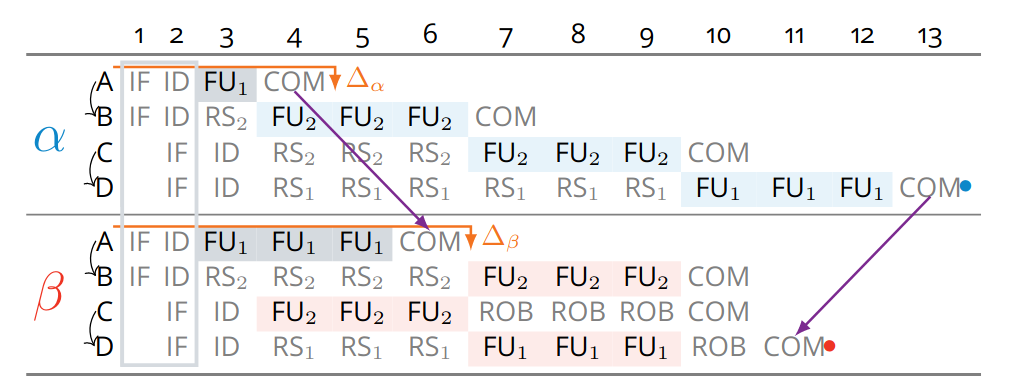
\includegraphics[width=\textwidth]{figures/step-func-good.png}
        \caption{Interpretation of example \ref{ex:simple-ta} using Gebhard's definition}
        \label{fig:step-good}
    \end{subfigure}
    \hfill
    \begin{subfigure}[t]{0.49\textwidth}
        \centering
        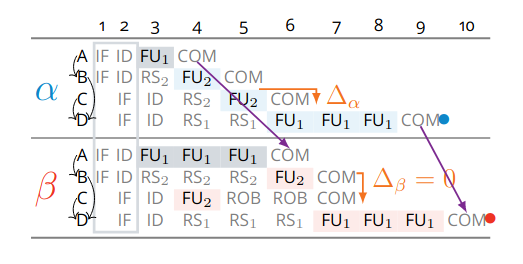
\includegraphics[width=\textwidth]{figures/step-func-bad.png}
        \caption{Counterexample to the definition}
        \label{fig:step-bad}
    \end{subfigure}
    \caption{Gebhard's definition applied to execution traces (from \cite{binder_definitions_2022})}
    \label{fig:step}
\end{figure}

In his thesis \cite{binder_definitions_2022}, Binder provides a counterexample (figure \ref{fig:step-bad}), where it is clear that there is no TA (trace $\beta$ has both unfavorable variation and longer execution time). However, Gebhard's definition signals an anomaly because of shorter local execution time of instruction $C$ in trace $\beta$.

This poses a question whether it is reasonable to capture a local execution time as difference between instruction completion times. 

\subsection{Step-functions Intersections}

\begin{figure}[H]
    \centering
    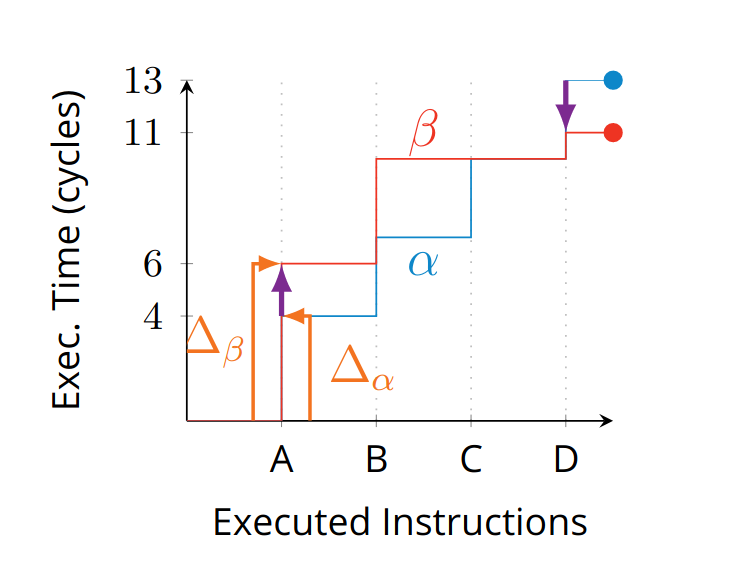
\includegraphics[width=0.6\textwidth]{figures/step-functions.png}
    \caption{Execution time as step functions (from \cite{binder_definitions_2022})}
    \label{fig:exec-time-step-fun}
\end{figure}

Similar definition is proposed by Cassez et al. \cite{cassez_what_2012}. The difference is that only global execution time is taken into account. Thus, TA arises when step-functions (that map instructions to their absolute completion time) of two traces intersect. For example, Figure \ref{fig:exec-time-step-fun} shows execution times as step functions from example \ref{ex:simple-ta}. The two functions intersect between $C$ and $D$ thus signalling an anomaly.

\begin{figure}[!htb]
    \centering
    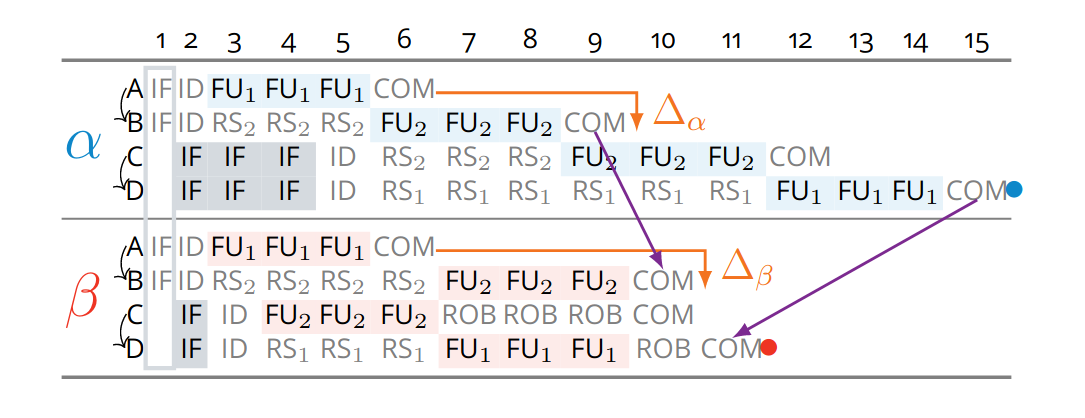
\includegraphics[width=\textwidth]{figures/step-func-2-bad.png}
    \caption{Contradicting result of Cassez's definition (from \cite{binder_definitions_2022})}
    \label{fig:step-2}
\end{figure}

This definition also leads to misleading effect with scenario found by Binder \cite{binder_definitions_2022}. Figure \ref{fig:step-2} illustrates this by comparing two traces. Step-functions of traces $\alpha$ and $\beta$ intersect, however there is no counter-intuitive TA happening as $\alpha$ is both longer and has a  longer latency for IF stage of instructions $C$ and $D$.

\subsection{Component Occupation}

An alternative approach is proposed by Kirner et al. \cite{kirner_precise_2009}. In their work the idea is to partition hardware into components and for each define the occupation by instruction (for how many cycles it processes the instruction). TA arises when a shorter component occupation coincides with a longer execution time in a chosen trace. For example, take Figure \ref{fig:step-good} and consider $FU_1$ and $FU_2$ as hardware components. In total, $FU_1$ is occupied for 4 cycles in trace $\alpha$ and 6 cycles in trace $\beta$. In the same time the execution time of $\alpha$ is longer, so a TA is identified.

A main challenge with this definition is choosing the right components. The authors do not give a formal way to define what a component is or what properties it should have. For example, in the previous case, it is not clear if the chosen partitioning is valid, since functional units like $FU_1$ and $FU_2$ are controlled by the processor's instruction scheduling and thus are not fully independent. Another problem is that the occupation time of a component can change because of instructions that are not directly related to the timing anomaly. For instance, an earlier or later instruction, which does not affect the total execution time, might still reduce the occupation time of a component and cause a false positive. Similarly, false negatives can also occur. Additionally, if a resource switch happens (for example, an instruction is executed on a different functional unit in another trace), it can make the comparison of occupation times unreliable and further complicate the detection of timing anomalies.

\TODO{counterexample}

% \subsection{Instruction Locality}


\TODO{Instruction Locality}

% \subsection{Progress-based definition}

\TODO{Progress-based definition}

Hahn and Reineke \cite{hahn_design_2020} introduce the notion of progress, ... \cite{gruin_minotaur_2023}

\subsection{Event Time Dependency Graph}

Binder et al. \cite{binder_definitions_2022} define TAs using the notion of causality between events in execution trace. In this work, superscalar OoO pipeline is considered. The processor state is described as a composition of states of each of the resource: \textit{IF, ID, set of RS, set of FU, ROB, COM}. Each component holds the information about instruction it is currently processing, including required registers and remaining clock cycles.

Notion of event is introduced based on qualitative changes in the pipeline associated to instruction progressing through stages. Event from execution trace (denoted as $e \in Events(\alpha$)) is a triple $(i,r,t)$, where $i$ is the instruction to which event is related, $r$ is the associated resource and the action (acquisition or release) and $t$ is a timestamp corresponding to the clock cycle when event occurs.

In the proposed framework events are related to \textit{IF, ID, FU} and \textit{COM} stages. For each instruction there are 7 types of events: $\IFa$, $\IFr$, $\IDa$, $\IDr$, $\FUa$, $\FUr$ and $COM$. $\uparrow$ signs the acquisition of a resource and $\downarrow$ its release. $COM$ denotes the acquisition of the commit stage; hence its release always happens one clock cycle after and no subsequent stages exist, it is not included into framework.

\textbf{Latency} is defined as the time difference between the acquisition and release of a resource. Each instruction passes through the same pipeline stages and is associated with corresponding events. Therefore, for each pair of traces corresponding to the same program, the sets of events differ only in their timestamps or, potentially, in the functional unit (FU) used (although resource switching is not modeled within this framework). Consequently, for each event in one trace, there exists a corresponding event in the other. Formally, this correspondence is defined by the function $CospEvent: Events(\alpha) \rightarrow Events(\beta)$.


A \textbf{variation} signs that the latency in one trace differs from latency of corresponding events in the other trace. On the pair of traces $\alpha$ and $\beta$. The variation is considered favorable for $\alpha$ if the latency in $\alpha$ is smaller than in $\beta$.

Variations are chosen as a source of timing anomalies. They may represent different memory behavior (cache hit or miss) for fetch and memory accesses in FU. Other sources of TA such as memory bus contention or branching are not considered by the framework.

\textbf{Event Time Dependency Graph (ETDG)} of trace $\tau$ denoted as $G(\tau) = (\mathcal{N}, \mathcal{A})$ is composed of a set of nodes $\mathcal{N} = Events(\tau)$ and a set of arcs $\mathcal{A} \subseteq \mathcal{N} \times \mathcal{N} \times \mathbb{N}$. 


Arc is a triple $(e_1, e_2, w)$ written as $e_1 \xrightarrow{w} e_2$ where $e_1$ is the source event node, $e_2$ -- destination node and $w$ is a lower bound of the delay between the two events. The arc means that at least $w$ clock cycles must pass between $e_1$ and $e_2$. 

Arcs are derived from a set of rules:
\begin{enumerate}
    \item \textbf{Order of pipeline stages}
    
    Every instruction goes through the pipeline stages in a fixed order: first it is fetched, then decoded, then executed and only then committed. This creates a following dependencies for a given instruction $I$:

    \begin{itemize}
        \item $(I, \IFr, t_1) \xrightarrow{0} (I, \IDa, t_2)$
        \item $(I, \IDr, t_3) \xrightarrow{0} (I, \FUa, t_4)$
        \item $(I, \FUr, t_5)  \xrightarrow{0} (I, COM, t_6)$
    \end{itemize}

    \item \textbf{Resource use}

    An instruction takes one or several clock cycles to go through each stage and cannot pass them faster.

    \begin{itemize}
        \item $(I, \IFa, t_0) \xrightarrow{lat_{IF}} (I, \IFr, t_1)$
        \item $(I, \IDa, t_2) \xrightarrow{1} (I, \IDr, t_3)$
        \item $(I, \FUa, t_4)  \xrightarrow{lat_{FU}} (I, \FUr, t_5)$
    \end{itemize}

    $lat_{IF}$ and $lat_{FU}$ are the latencies of IF and FU stages respectively.

    $lat_{IF} = t_1 - t_0$, $lat_{FU} = t_5 - t_4$

    \item \textbf{Instruction order}
    
    In-order part of the pipeline is constrained by instruction order. Thus, for successive instructions $I_1$ and $I_2$:

    $(I_1, RES\uparrow, t) \xrightarrow{0} (I_2, RES\uparrow, t'), RES \in \{IF, ID, COM\}$


    \item \textbf{Data dependencies}
    
    RAW dependency between $I_1$ and $I_2$ restricts the execution order of the instructions:  $(I_1, \FUr, t) \xrightarrow{0} (I_2, \FUa, t')$.
    
    \item \textbf{Resource contention}
    
    Also some instruction can be delayed because of limited resources. For instance, FU contention happens when $I_1$ and $I_2$ use the same FU, and it is busy by $I_1$ at the moment when $I_2$ is ready. This creates $(I_1, \FUr, t) \xrightarrow{0} (I_2, \FUa, t')$. 

    Resource contention can also be caused by reaching the capacity limit of ROB or RS. 
\end{enumerate}

\textbf{Causality graph} is achieved from ETDG by removing unnecessary edges. For each event we keep only the most relevant constraint. Only arcs of the form $e_1 \xrightarrow{e_2.time - e_1.time} e_2$ are left. Also arcs related to variations are excluded.

\textbf{Timing anomaly} according to Binder consists of three observations: variation, causality and slowdown. If a trace exhibits a favorable variation and in a causal region there is an event which is delayed, then TA is signalled.

Formally, TA is observed on pair of traces $\alpha$ and $\beta$ if there exists a favorable variation in $\alpha$ relative to $\beta$. Let $\downarrow e_\alpha$ and $\downarrow e_\beta$ be the events corresponding to the end of the variation in both traces. If there exist events $e'_\alpha$ and $e'_\beta$, where $e'_\beta = CospEvent(e'_\alpha)$ and there is a path in causality graph of $\alpha$ between $\downarrow e_\alpha$ and $e'_\alpha$, s.t. $\Delta(\downarrow e_\beta,e'_\beta) < \Delta(\downarrow e_\alpha,e'_\alpha)$.



\begin{figure}[htbp]
    \centering
    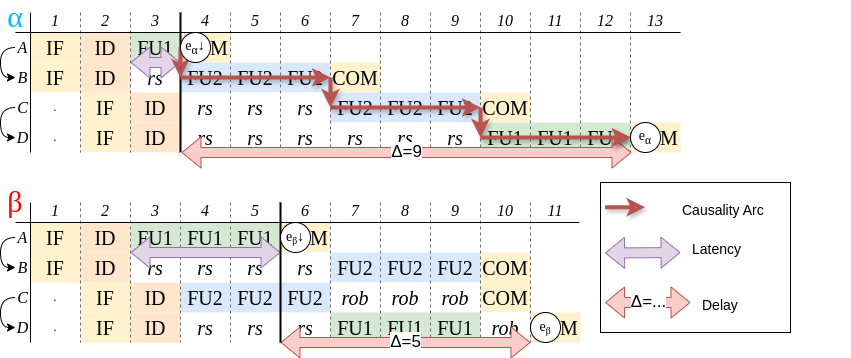
\includegraphics[width=0.8\textwidth]{figures/multiscalar_ta_causality.png}
    \caption{Causality-based TA detection applied to Example \ref{ex:simple-ta}. $e_\alpha\downarrow = (A, \FUr, 4), e_\beta\downarrow = (A, \FUr, 6), e_\alpha = (A, COM, 13), e_\beta = (A, COM, 11)$. Purple arrow denotes latency which has a variation between two traces. Gray arrow shows delay between events which is greater in favorable trace. Causality in  path $\alpha$ is marked by red arrows.}
    \label{fig:multiscalar-ta-causality}
\end{figure}

\begin{figure}[htbp]
    \centering
    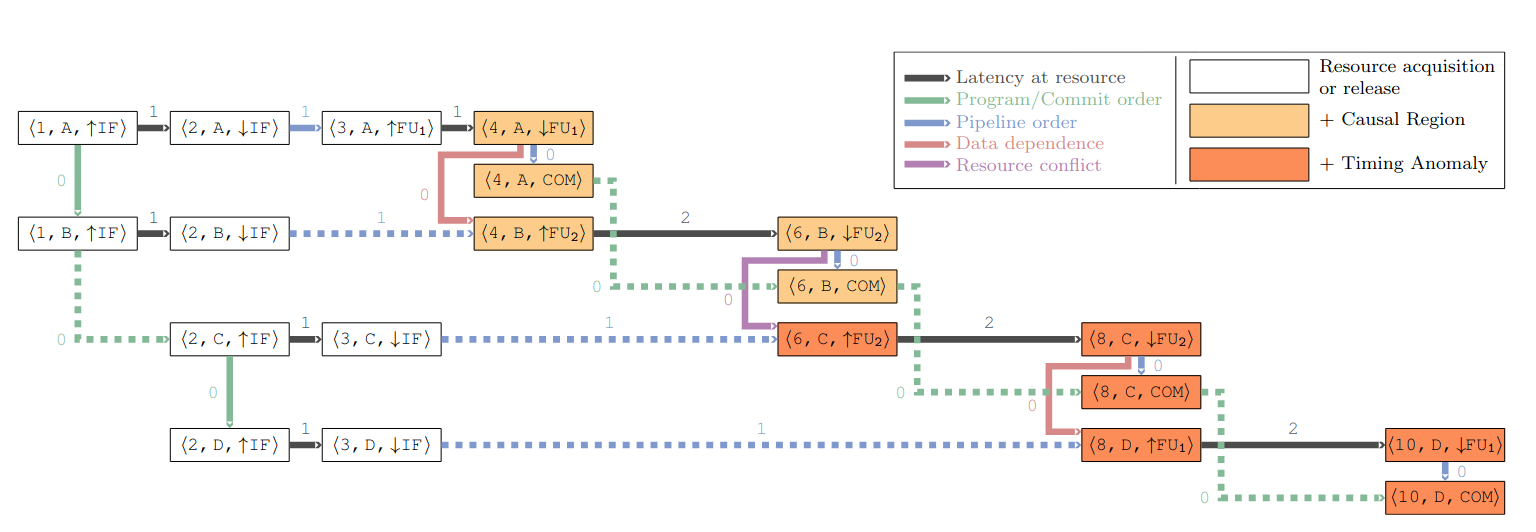
\includegraphics[width=\textwidth]{figures/ETDG.png}
    \caption{Complete ETDG for trace $\alpha$ from Figure \ref{fig:multiscalar-ta-causality}, trace $\alpha$. \TODO{image source}}
    \label{fig:ETDG}
\end{figure}

Figure \ref{fig:multiscalar-ta-causality} shows how the framework captures TA for example \ref{ex:simple-ta}. Figure \ref{fig:ETDG} presents the complete ETDG for trace $\alpha$ with different dependency rules highlighted with different colors. The arcs reflecting causality are depicted in solid lines.

In contrast to other definition, this one measures relative time from the acquisition of the resource instead of global time. This approach allows the separation of different variations and isolates the part of the trace that experiences TA-effect.


\section{TA-classifications}

